\subsubsection{MSVC: x86}

\lstinputlisting{patterns/04_scanf/ex2_MSVC.asm}

\IFRU{Ничего особенного, в целом. Теперь \TT{x} объявлена в сегменте \TT{\_DATA}. 
Память для нее в стеке более не выделяется.
Все обращения к ней происходит не через стек, а уже напрямую. 
Неинициализированные глобальные переменные не занимают места в исполняемом файле
(и действительно, зачем в исполняемом файле
нужно выделять место под изначально нулевые переменные?), но тогда, когда к этому месту в памяти
кто-то обратится, \ac{OS} подставит туда блок состоящий из нулей\footnote{Так работает \ac{VM}}.}
{Now \TT{x} variable is defined in the \TT{\_DATA} segment. 
Memory in local stack is not allocated anymore. 
All accesses to it are not via stack but directly to process memory. 
Not initialized global variables takes no place in the executable file
(indeed, why we should allocate a place
in the executable file for initially zeroed variables?), but when someone will access this place
in memory, \ac{OS} will allocate a block of zeroes there\footnote{That is how \ac{VM} behaves}.}

\IFRU{Попробуем изменить объявление этой переменной:}
{Now let's assign value to variable explicitly:}

\begin{lstlisting}
int x=10; // default value
\end{lstlisting}

\IFRU{Выйдет в итоге:}{We got:}

\begin{lstlisting}
_DATA	SEGMENT
_x	DD	0aH

...
\end{lstlisting}

\IFRU{Здесь уже по месту этой переменной записано \TT{0xA} с типом DD (dword = 32 бита).}
{Here we see value \TT{0xA} of DWORD type (DD meaning DWORD = 32 bit).}

\IFRU{Если вы откроете скомпилированный .exe-файл в \IDA, то увидите что \IT{x} 
находится аккурат в начале сегмента \TT{\_DATA}, после этой переменной будут текстовые строки.}
{If you will open compiled .exe in \IDA, you will see the \IT{x} variable placed at the beginning of 
the \TT{\_DATA} segment, and after you'll see text strings.}

\IFRU{А вот если вы откроете в \IDA, .exe скомпилированный в прошлом примере, 
где значение \IT{x} не определено, то в IDA вы увидите:}
{If you will open compiled .exe in \IDA from previous example where \IT{x} value is not defined, 
you'll see something like this:}

\begin{lstlisting}
.data:0040FA80 _x              dd ?                    ; DATA XREF: _main+10
.data:0040FA80                                         ; _main+22
.data:0040FA84 dword_40FA84    dd ?                    ; DATA XREF: _memset+1E
.data:0040FA84                                         ; unknown_libname_1+28
.data:0040FA88 dword_40FA88    dd ?                    ; DATA XREF: ___sbh_find_block+5
.data:0040FA88                                         ; ___sbh_free_block+2BC
.data:0040FA8C ; LPVOID lpMem
.data:0040FA8C lpMem           dd ?                    ; DATA XREF: ___sbh_find_block+B
.data:0040FA8C                                         ; ___sbh_free_block+2CA
.data:0040FA90 dword_40FA90    dd ?                    ; DATA XREF: _V6_HeapAlloc+13
.data:0040FA90                                         ; __calloc_impl+72
.data:0040FA94 dword_40FA94    dd ?                    ; DATA XREF: ___sbh_free_block+2FE
\end{lstlisting}

\IFRU{\TT{\_x} обозначен как \TT{?}, наряду с другими переменными не требующими инициализации. 
Это означает, что при загрузке .exe в память, место под все это выделено будет. 
Но в самом .exe ничего этого нет. Неинициализированные переменные не занимают места в исполняемых файлах. Удобно для больших массивов, например.}
{\TT{\_x} marked as \TT{?} among other variables not required to be initialized. 
This means that after loading .exe to memory, a space for all these variables will be 
allocated and a random garbage will be here. 
But in an .exe file these not initialized variables are not occupy anything. 
E.g. it is suitable for large arrays.}

\subsubsection{MSVC: x86 + \olly}
\index{\olly}

\IFRU{Тут даже проще}{Things are even simpler here}: \figname \ref{fig:scanf_ex2_olly_1}.
\IFRU{Переменная хранится в сегменте данных}{Variable is located in the data segment}.
\IFRU{Кстати, после исполнения инструкции \PUSH, заталкивающей адрес $x$, адрес появится в стеке, и на этом
элементе можно нажать правой кнопкой, выбрать ``Follow in dump''}{By the way, after 
\PUSH instruction, pushing $x$ address, is executed, the address
will appear in stack, and it is possible to right-click on that element and select ``Follow in dump''}.
\IFRU{И в окне памяти слева появится эта переменная}{And the variable will appear in the memory window
at left}.

\IFRU{После того как в консоли введем 123, здесь появится}{After we enter 123 in the console,} 
\TT{0x7B}\EN{ will appear here}.

\IFRU{Почему самый первый байт это}{But why the very first byte is} \TT{7B}?
\IFRU{По логике вещей, здесь должно было бы быть}{Thinking logically, a} \TT{00 00 00 7B}\EN{ should be
there}.
\IFRU{Это называется}{This is what called} \gls{endianness}, \IFRU{и в x86 принят формат}{and} 
\IT{little-endian}\EN{ is used in x86}.
\IFRU{Это означает что в начале записывается самый младший байт, а заканчивается самым старшим байтом}
{This mean that lowest byte is written first, and highest written last}.
\IFRU{Больше об этом}{More about it}: \ref{sec:endianness}.

\IFRU{Позже, из этого места в памяти, 32-битное значение загружается в \EAX и передается в}
{Some time after, 32-bit value from this place of memory is loaded into \EAX and passed into} \printf.

\IFRU{Адрес переменной $x$ в памяти}{$x$ variable address in the memory is} \TT{0xDC3390}.
\IFRU{В \olly{} мы можем посмотреть карту памяти процесса (Alt-M) и увидим что этот адрес
внутри PE-сегмента \TT{.data} нашей программы}{In \olly we can see process memory map (Alt-M)
and we will see that this address is inside of \TT{.data} PE-segment of our program}:
\figname \ref{fig:scanf_ex2_olly_2}.

\begin{figure}[H]
\centering
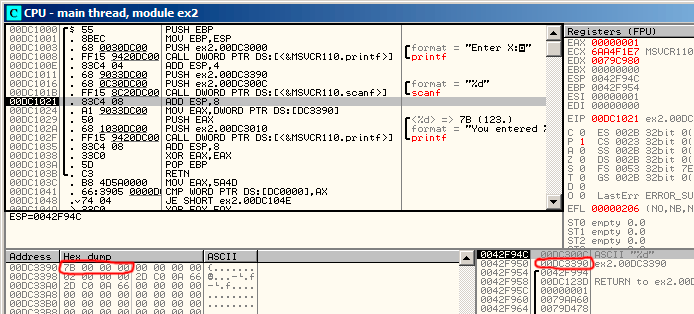
\includegraphics[scale=0.66]{patterns/04_scanf/ex2_olly_1.png}
\caption{\olly: \IFRU{после исполнения \scanf}{after \scanf execution}}
\label{fig:scanf_ex2_olly_1}
\end{figure}

\begin{figure}[H]
\centering
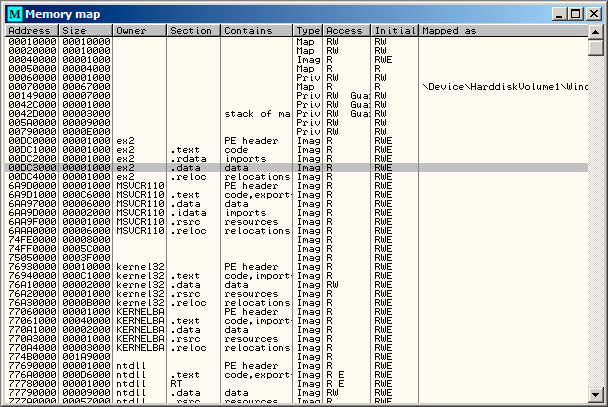
\includegraphics[scale=0.66]{patterns/04_scanf/ex2_olly_2.png}
\caption{\olly: \IFRU{карта памяти процесса}{process memory map}}
\label{fig:scanf_ex2_olly_2}
\end{figure}

\subsubsection{GCC: x86}

\index{ELF}
\IFRU{В Linux все также почти. За исключением того, что если значение \TT{x} не определено, 
то эта переменная будет находится в сегменте \TT{\_bss}.
В \ac{ELF} этот сегмент имеет такие атрибуты:}
{It is almost the same in Linux, except segment names and properties: 
not initialized variables are located in the \TT{\_bss} segment. 
In \ac{ELF} file format this segment has such attributes:}

\begin{lstlisting}
; Segment type: Uninitialized
; Segment permissions: Read/Write
\end{lstlisting}

\IFRU{Ну а если сделать статическое присвоение этой переменной какого-либо
значения, например, $10$, то она будет находится 
в сегменте \TT{\_data},
это сегмент с такими атрибутами:}
{If to statically assign a value to variable, e.g. $10$, it will be placed in the \TT{\_data} segment, 
this is segment with the following attributes:}

\begin{lstlisting}
; Segment type: Pure data
; Segment permissions: Read/Write
\end{lstlisting}

\subsubsection{MSVC: x64}

\lstinputlisting[caption=MSVC 2012 x64]{patterns/04_scanf/ex2_MSVC_x64.asm}

\IFRU{Почти такой же код как и в}{Almost the same code as in} x86.
\IFRU{Обратите внимание что для \TT{scanf()} адрес переменной $x$ передается
при помощи инструкции \LEA, а во второй \printf передается само значение переменной при помощи \MOV}
{Take a notice that $x$ variable address is passed to \TT{scanf()} using \LEA instruction,
while the value of variable is passed to the second \printf using \MOV instruction}.
\TT{``DWORD PTR''}\EMDASH{}\IFRU{это часть языка ассемблера (не имеющая отношения к машинным кодам) 
показывающая, что тип переменной в памяти\EMDASH{}именно 32-битный, 
и инструкция \MOV должна быть здесь закодирована соответственно}{is a part of assembly language 
(no related to machine codes), showing that the variable data type is 32-bit and the \MOV instruction
should be encoded accordingly}.


